\begin{figure}[th]
\centering
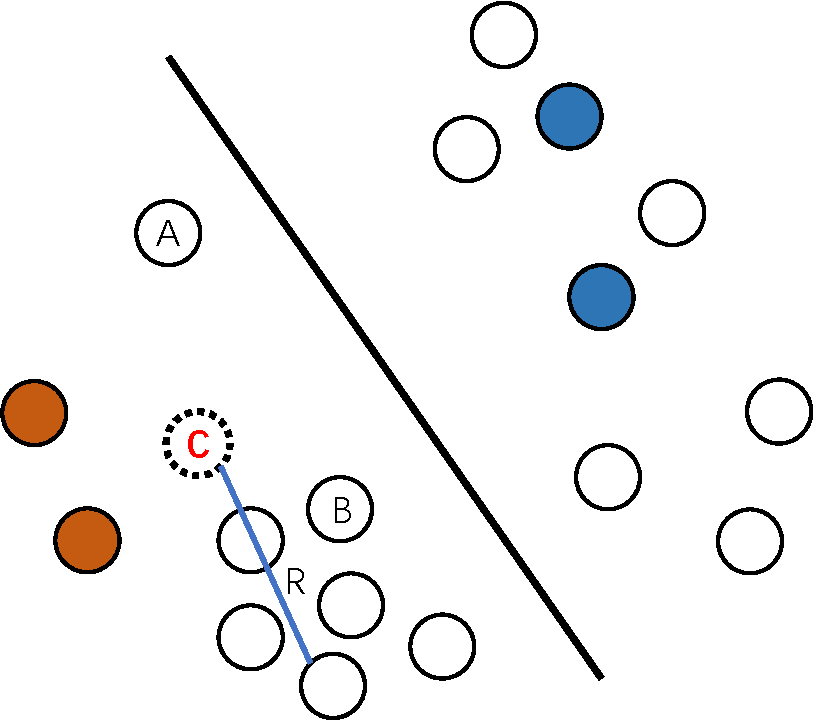
\includegraphics[scale=0.3]{figs/radius.pdf}
\caption{Geometric meaning of radius. Points on the left and points on the right
belong to different classes. A, B are data points and C is the hypothesis center. 
R denotes the maximum Euclidean distance between C and points on the left.}
\label{fig:radius}
\end{figure}


\section{Approach}
\label{sec:appraoch}
In this section, we propose two new techniques. We model the representative of a sample
point in a different way. To solve oversampling problem in many-class classification task, we utilize frequency of predicted class in the label pool to smooth the scoring function $\mathcal{V}(x)$.

\subsection{Uncertainty with Class Radius}
We want to utilize $\mathcal{X}$ to improve the sampling quality. 
WU also takes into account $\mathcal{X}$ but depends too much on the 
intermediate classifier output. It calculates the distance
between unlabeled data point and center. 
However, the classifier trained at the early stage
is inaccurate and the hidden vectors are not reliable. 
So the distance will be quite different from the true distance. 
In order to alleviate the distraction by such immature classifiers, we relax the condition of evaluating the representative of each point and define class radius score $\mathcal{R}(\hat{y_i}=k|x_i)$ to measure the value of each class. 
%Like weighted uncertainty, we combine the uncertainty along with radius score.
    
$$ \mathcal{V}(x_i) = \mathcal{H}(x_i) \mathcal{R}(\hat{y_i}=k|x_i)$$
    
The radius score $\mathcal{R}(\hat{y_i}=k|x_i)$ can be calculated as follows. First, we obtain the hypothesis center point of each class by averaging the feature vector of all data points classified into this class. We define radius as the maximum Euclidean distance between center point and points belonging to this class. Figure \ref{fig:radius} shows the geometric meaning of radius.
    $$C_k = \frac{1}{|\mathcal{U}_k|} \sum_{x_j \in \mathcal{U}_k} h(x_j)$$
    $$\mathcal{R}(\hat{y_i}=k|x_i) = \max_{x_j \in \mathcal{U}_k} \sqrt{||x_j - C_k||_2} $$
    
Instead of querying representative and informative points, we tend to choose points which can reduce the class radius to the most extent. In other words, we hope to equally discover the unlabeled feature space by selecting a point whose class radius is large. In many-class classification, the objective is to make it easier for classifier to extract the feature of each class so that the performance will increase significantly. Moreover, since many points may share the same radius score, we combine it with uncertainty score such that we can select point that is uncertain as well as its predicted class is also uncertain to the classifier.
    
 WU relies too much on the classifier, and any small noises will change the center and thus amplifies the change on the similarity scores on some points, while our proposed approach is more robust since slight changes of the center position in most cases will not influence on a class with large radius.
    
\subsection{Adjustment on Class Frequency}
The increase of classes causes the decrease of performance for
current AL methods, because they mostly consider binary classification problems, 
often causing over-sampling of one single class. However, for many-class classification tasks, over-sampling of certain classes will lead to dramatic decrease in performance. Take an extreme situation as example, for a 50-class classification tasks, if we only query one class and obtains 1 in this class, the overall macro F1 is still disappointing 0.02. In order to solve this problem, we add a frequency adjustment feature 
$\mathcal{F}$ which can be combined with most probability-based AL methods
including all the methods we introduced earlier.
$$\mathcal{V}'(x_i) = \mathcal{F}(\hat{y}_i|x_i) \mathcal{V}(x_i)$$    
The frequency score $\mathcal{F}$ can be calculated as:
$$\mathcal{F}(\hat{y_i} = y_k|x_i) = \frac{1}{|\mathcal{L}_k|}$$    
where $\mathcal{L}_k$ is the labeled set of label $k$.
    
    
Also, to avoid diminishing utility score when the frequency is too large,
we can smooth feature using square root or logarithm function. 
The tuned frequency score can be calculated as: 
    $$\mathcal{F}(\hat{y_i} = y_k|x_i) = \frac{1}{\log{|\mathcal{L}_k|}}$$    
    $$\mathcal{F}(\hat{y_i} = y_k|x_i) = \frac{1}{\sqrt{|\mathcal{L}_k|}}$$    
    
%Next, we will evaluate these two techniques. 
